\documentclass[nobib]{tufte-handout}

%\\geometry{showframe}% for debugging purposes -- displays the margins

\newcommand{\bra}[1]{\left(#1\right)}
\usepackage{clrscode3e}
\usepackage{hyperref}
\usepackage[activate={true,nocompatibility},final,tracking=true,kerning=true,spacing=true,factor=1100,stretch=10,shrink=10]{microtype}
\usepackage{color}

% Fixes captions and images being cut off
\usepackage{marginfix}

\usepackage{circuitikz}
\usepackage{siunitx}
\usepackage{amsmath,amsthm}
\usetikzlibrary{shapes}
\usetikzlibrary{positioning}
\usetikzlibrary{arrows}

% Set up the images/graphics package
\usepackage{graphicx}
\setkeys{Gin}{width=\linewidth,totalheight=\textheight,keepaspectratio}
\graphicspath{{.}}

\title{Notes for ECE 20001 - EE Fundementals I}
\author[Ezekiel Ulrich]{Ezekiel Ulrich}
\date{\today}  % if the \date{} command is left out, the current date will be used

% The following package makes prettier tables.  We're all about the bling!
\usepackage{booktabs}

% The fancyvrb package lets us customize the formatting of verbatim
% environments.  We use a slightly smaller font.
\usepackage{fancyvrb}
\fvset{fontsize=\normalsize}

% Small sections of multiple columns
\usepackage{multicol}

% These commands are used to pretty-print LaTeX commands
\newcommand{\doccmd}[1]{\texttt{\textbackslash#1}}% command name -- adds backslash automatically
\newcommand{\docopt}[1]{\ensuremath{\langle}\textrm{\textit{#1}}\ensuremath{\rangle}}% optional command argument
\newcommand{\docarg}[1]{\textrm{\textit{#1}}}% (required) command argument
\newenvironment{docspec}{\begin{quote}\noindent}{\end{quote}}% command specification environment
\newcommand{\docenv}[1]{\textsf{#1}}% environment name
\newcommand{\docpkg}[1]{\texttt{#1}}% package name
\newcommand{\doccls}[1]{\texttt{#1}}% document class name
\newcommand{\docclsopt}[1]{\texttt{#1}}% document class option name

% Define a custom command for definitions
\newcommand{\defn}[2]{\noindent\textbf{#1}:\ #2}

\begin{document}

\maketitle

\begin{abstract}
These are lecture notes for fall 2023 ECE 20001 at Purdue. Modify, use, and distribute as you please.
\end{abstract}

\tableofcontents

\section{Course Introduction}

This course covers fundamental concepts and applications 
for electrical and computer engineers as well as for engineers
 who need to gain a broad understanding of these disciplines. 
 The course starts by the basic concepts of charge, current, 
 and voltage as well as their expressions with regards to 
 resistors and resistive circuits. Essential concepts, 
 devices, theorems, and applications of direct-current (DC), 
 1st order, and alternating-current (AC) circuits are 
 subsequently discussed. Besides electrical devices and 
 circuits, basic electronic components including diodes and 
 transistors as well as their primary applications are also 
 discussed. For more information, see the syllabus. 

\section{Equations}

\begin{enumerate}
    \item $P = \frac{dW}{dt} = IV$
    \item $I = \frac{dq}{dt}$
    \item $V = \frac{W}{q}$
    \item $R = \frac{\rho L}{A}$
    \item Ohm's Law: $V=IR$
    \item Coulomb's Law: $\vec{F} = \frac{1}{4\pi \epsilon_0}\frac{q_1 q_2}{r^2}\hat{r}$
    \item Kirchhoff's Voltage Law: 
    \item Conductance: $G = \frac{1}{R}$
    \item Equivalent resistance: $R_{eq} = \frac{V_{test}}{I_{test}}$
\end{enumerate}

\pagebreak

\section{Charge, current, voltage, and power}
Before we begin a discussion
of electrical engineering, we will want an
understanding of some important concepts. 

\defn{Charge}{A fundemental property of matter.} Charge
is measured in units of Coulombs (C) and 
arises from aggregates of charged 
fundemental particles like electrons.

\defn{Current}{The rate of flow of charge.} Typically,
we think of current as occuring in a circuit, a loop
through which charge can flow. Current can
be mathematically defined as $I = \frac{dq(t)}{dt}$, where 
$q(t)$ is the charge at time $t$. Current therefore has units
of Coulombs per second (C/s). 

\defn{Voltage}{The difference in electric potential energy
between two points, per unit charge.} Voltage thus has units of
$\frac{J}{C}$. or Volts (V).
Intuitively, a stronger voltage source (such
as a battery) will result in a higher current on 
identical wires. Imagine a voltage source
as a concentration of negative charges on
one side and positive charges on the other. 
If we hook both ends up to a conducting wire and place 
an electron in the wire, it will be repelled 
from the negative side and attracted to the
positive side. The electron has a high
potential energy near the concentration of
negative charge, and a low potential energy
near the positive charges. The difference
between these potentials is the voltage. This should
make it clear that voltage must always be
defined as across two points, each with its
electric potential. A good note is that
voltage can be negative (if the electric 
potential at the second point measured is higher)
and it may not be constant with time. 

\defn{Power}{The rate of doing work, or changing energy.} 
Mathematically, $P = \frac{dW}{dt} = IV$ and has units of Watts (W).
In a closed system, power is always balanced: whatever 
is put out by sources is consumed by
loads. Thus, in a closed circuit, $\sum P = 0$ This
is an important point, so allow me to illustrate it with 
an example. Say we have the below circuit:

\begin{circuitikz} \draw
    (0,-2) -- (0,2)
      (0,2) -- (3,2)
      (3, 2) -- (3, 0)
      (0, -2) -- (9, -2)
      (0, 0) -- (9,0)
      (3, -2) -- (3, 0)
      (6, -2) -- (6, 0)
      (9, -2) -- (9, 0)
    ;
    \node[draw, rectangle, minimum width=0.5cm, minimum height=0.5cm] at (1.5,2) {G}
    (1.5,2.25) node[above] {$+ 4 V -$}

    (1.5,2) to [short,i=$1A$] (0,2);

    \node[draw, rectangle, minimum width=0.5cm, minimum height=0.5cm] at (1.5,0) {B}
    (1.5,0.25) node[above] {$+ 4 V -$}

    (0,0) to [short,i=$4A$] (1.5,0);

    \node[draw, rectangle, minimum width=0.5cm, minimum height=0.5cm] at (0,-1) {A}
    (-.25,-1) node[label={[rotate=90]above:$- 10V +$}] {};

    \draw (0,-.25) to[short, i=$3A$] (0, 0);

    \node[draw, rectangle, minimum width=0.5cm, minimum height=0.5cm] at (3,-1) {C}
    (2.75,-1) node[label={[rotate=90]above:$- 6V +$}] {};

    \draw (3,0) to[short, i=$5A$] (3, -.25);

    \node[draw, rectangle, minimum width=0.5cm, minimum height=0.5cm] at (6,-1) {E}
    (5.75,-1) node[label={[rotate=90]above:$+ 2V -$}] {};

    \draw (6,0) to[short, i=$-1A$] (6, -.25);

    \node[draw, rectangle, minimum width=0.5cm, minimum height=0.5cm] at (4.5,0) {D}
    (4.5,.25) node[above] {$+ 8V -$};

    \draw (3,0) to[short, i=$-2A$] (4.5, 0);

    \node[draw, rectangle, minimum width=0.5cm, minimum height=0.5cm] at (9,-1) {F}
    (8.75,-1) node[label={[rotate=90]above:$- 2V +$}] {};

    \draw (9,-1) to[short, i=$I$] (9, 0);

\end{circuitikz}

We know $\sum P_i = \sum V_i I_i = 0$. Let's keep track 
of each $P_i$ in a table, not forgetting passive
sign convention:
\begin{table}[ht]
    \centering
    \begin{tabular}{|c c|}
    \hline
    Symbol & Watts \\
    \hline
    $P_A$ & -30 \\
    $P_B$ & 16 \\ 
    $P_C$ & 30 \\
    $P_D$ & -16 \\
    $P_E$ & 2 \\
    $P_F$ & -2$I$ \\
    $P_G$ & -4 \\
    \hline
    \end{tabular}
    \caption{Power absorbed}
    \label{tab:powerabsorbtable}
\end{table}
Summing the rows of this table, we have 
$\sum P_i = 2I - 2 = 0$, implying $I = 1$.

In the previous example, we had current flowing
both into and out of the positive terminals
of elements. We also had negative currents. Let's define 
how to handle signage in circuits:

\defn{Passive sign convention}{Defines current as going into 
positive voltage node of a component.} The component
is labeled a \emph{load} or a \emph{passive device}.
We call it this because the component
consumes power. If a current is negative,
it is flowing in the opposite direction shown by the
arrow.
\begin{marginfigure}
    \centering
    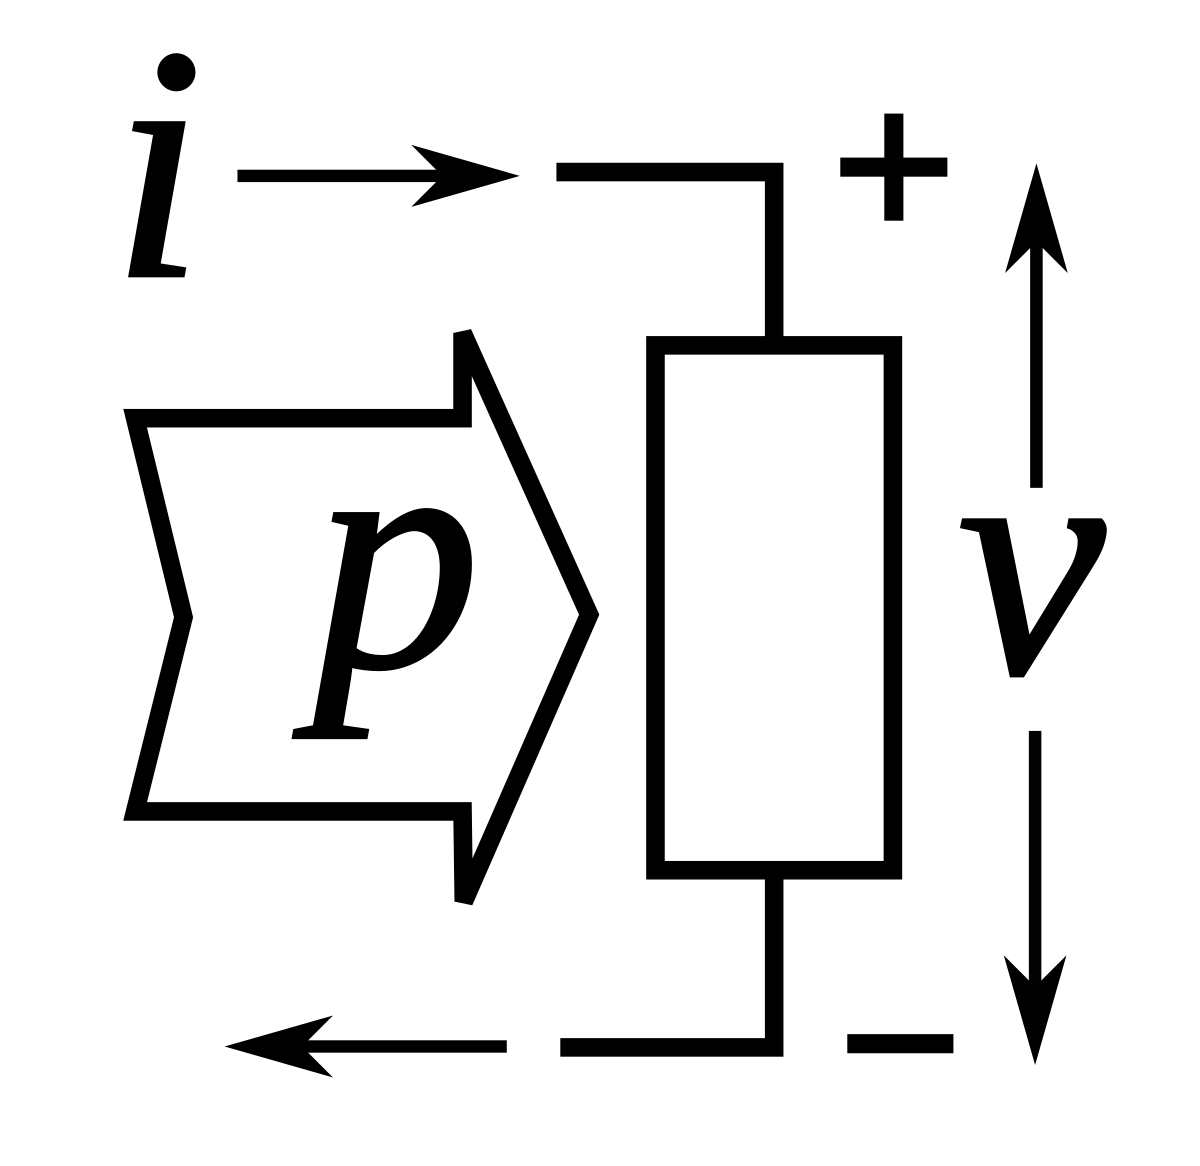
\includegraphics{images/Passive_sign_convention.svg.png}
    \caption{Passive sign convention}
    \label{fig:psc} 
\end{marginfigure}
It's useful to have an idea of the components of circuit
schematics (visual representations of a circuit). Below is a list 
of the terms that will be used in this course:
\begin{itemize}
    \item Elements: The term elements means "components and sources."
    \item Symbols: Elements are represented in schematics by symbols. 
    Symbols for common 2-terminal elements are displayed to the right.
    
\begin{marginfigure}
    \centering
    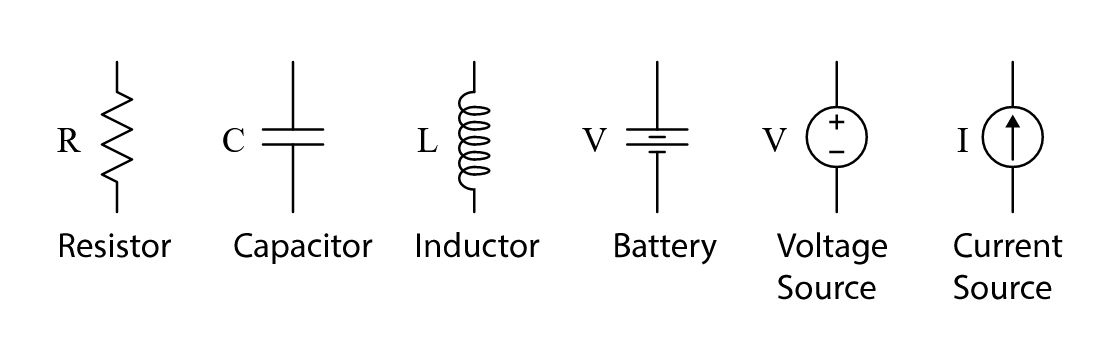
\includegraphics{images/symbols.png}
    \caption{Common circuit symbols}
    \label{fig:symbols}
\end{marginfigure} 

    \item Lines: Connections between elements are drawn as lines, 
    which we often think of as "wires". On a schematic, 
    these lines represent perfect conductors with zero resistance. 
    Every component or source terminal touched by a line is at the same voltage.
    \item Dots: Connections between lines can be indicated by dots. 
    Dots are an unambiguous indication that lines are connected. 
    If the connection is obvious, you don't have to use a dot.
\end{itemize}
Check out the circuit schematic below and see how many components you 
can identify!
\begin{center}
    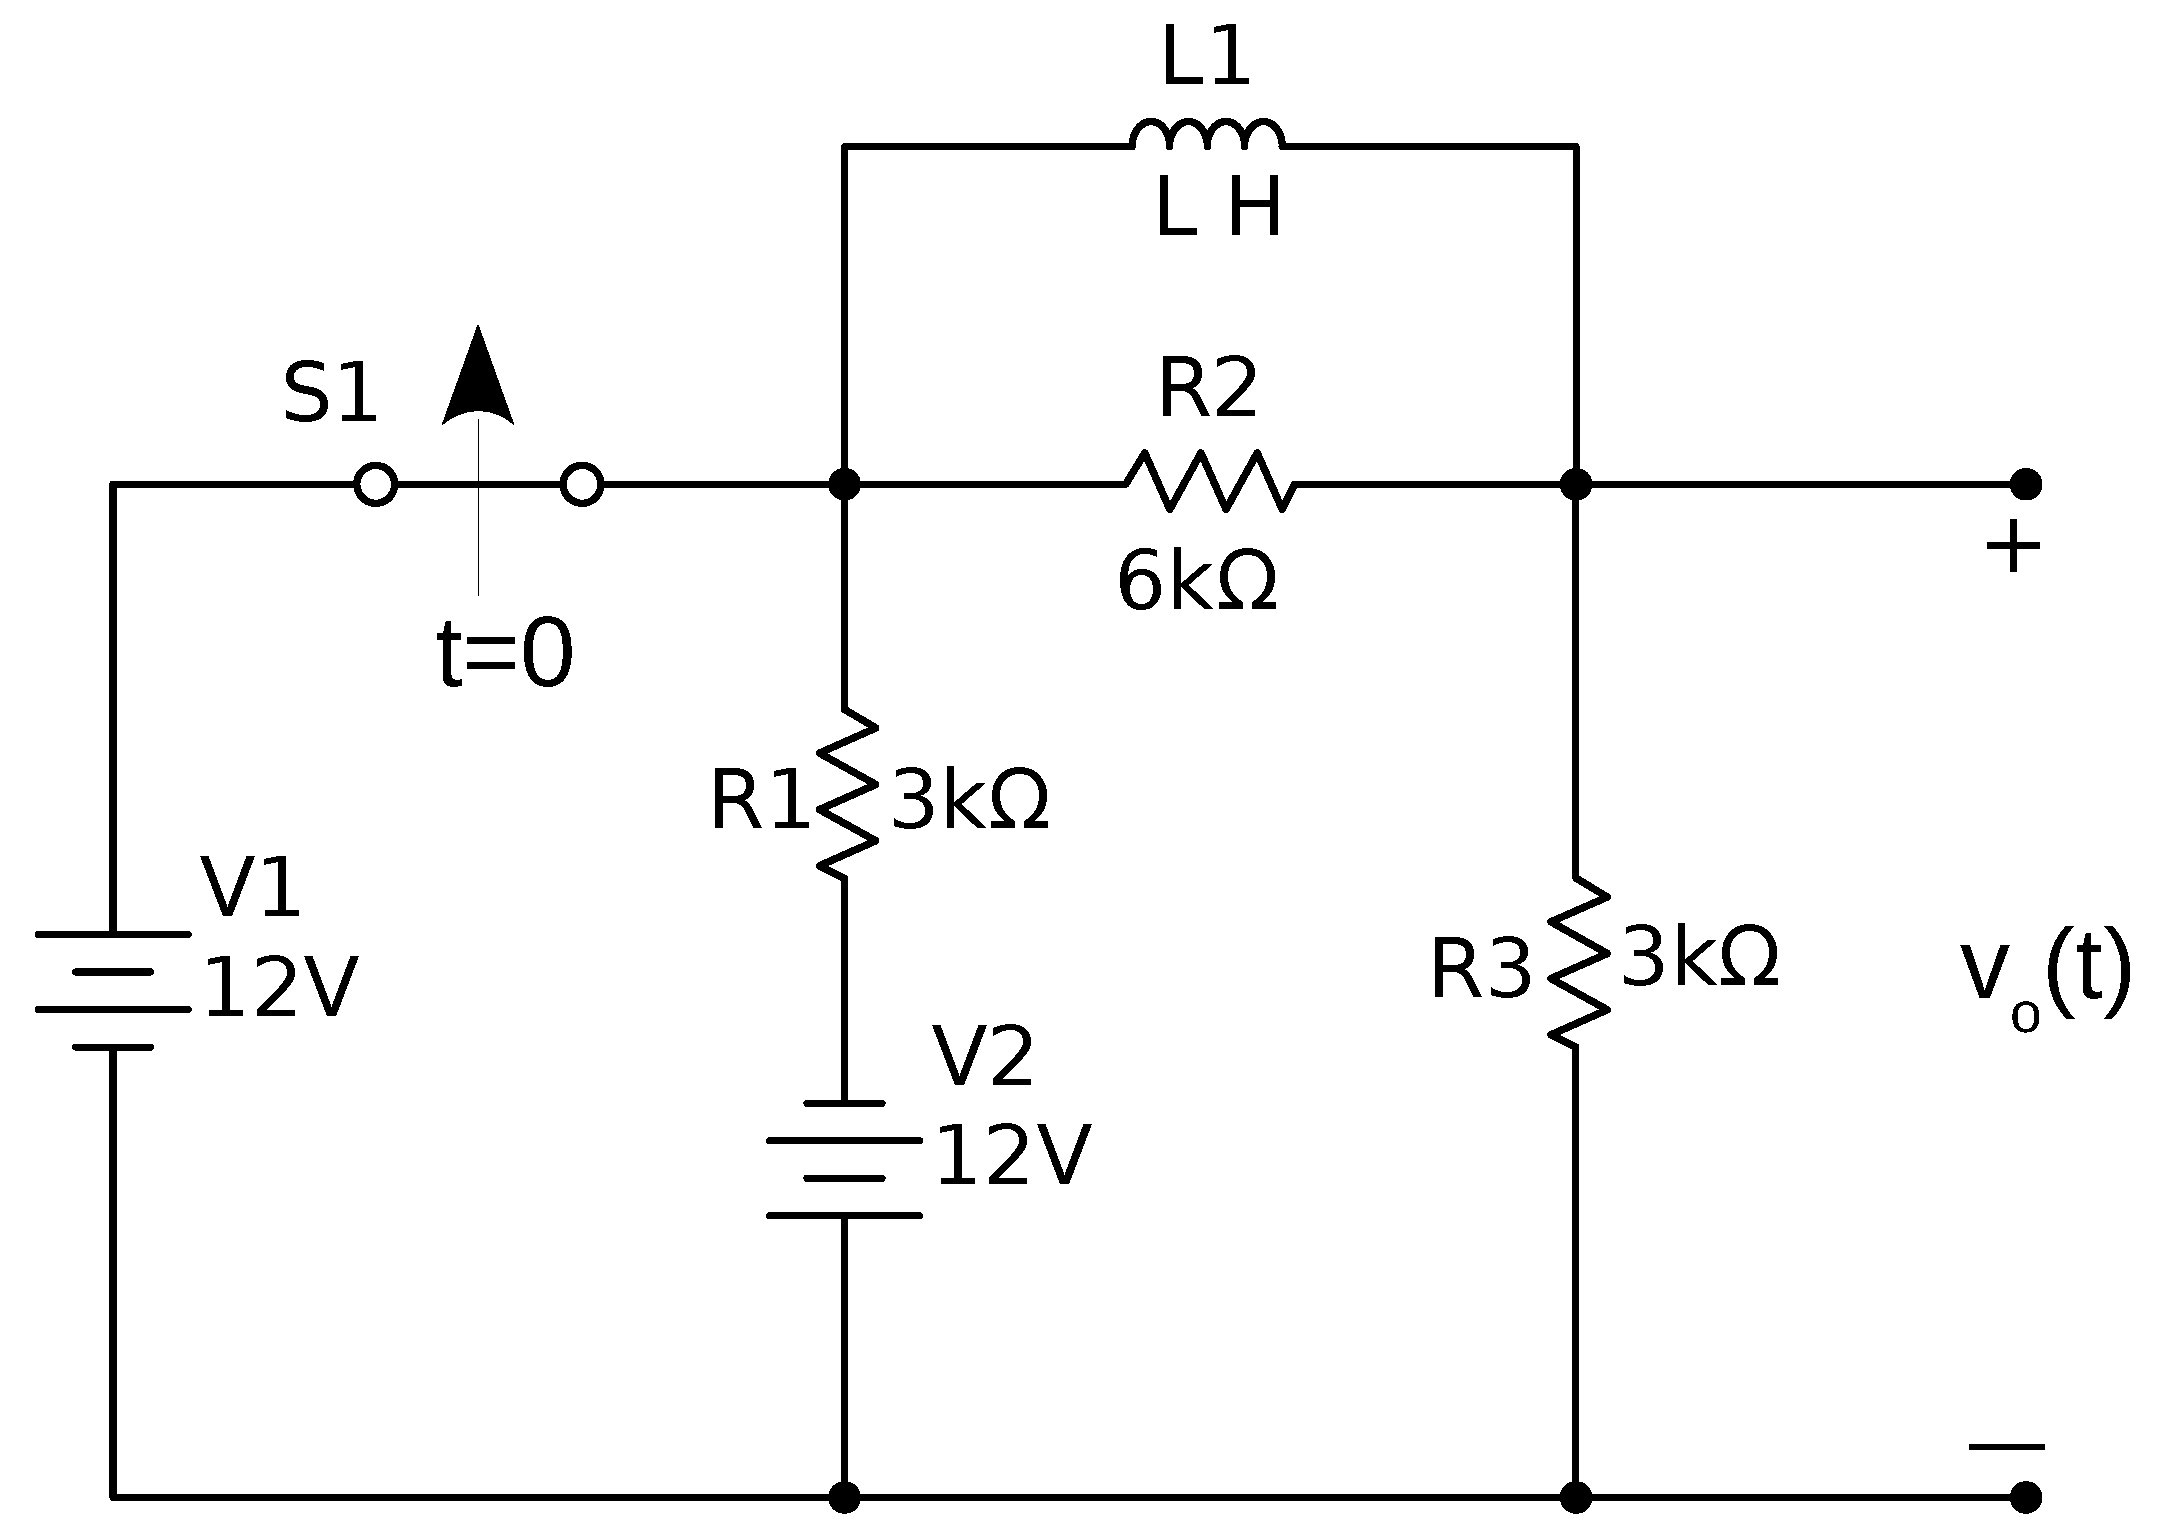
\includegraphics[width=\textwidth/2]{images/PS0_CapacitorCircuit.png}
\end{center}

\section{(In)dependent sources, connections, resistance and Ohm's Law}
Now, on to what circuits are doing. For interesting things
to happen we need electrons flowing through those wires,
and for that we need sources. There are two types: independent and dependent.
Independent sources are voltage sources or current sources 
that maintain a constant value regardless of the rest of the 
circuit. They are not influenced by the circuit's current or 
voltage conditions. There are two main types of independent 
sources:
\begin{itemize}
    \item \defn{Independent voltage source}{Maintains a constant 
    voltage across its terminals, regardless of the current 
    flowing through it. It is typically represented by a 
    symbol with a plus sign and a minus sign, indicating 
    the polarity of the voltage.} A battery maintaining a constant
    voltage of 9 V is an example of an independent voltage source.
    \begin{marginfigure}
        \centering
        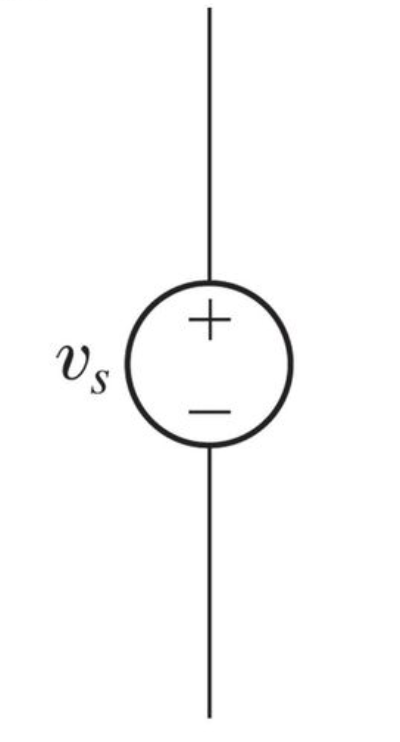
\includegraphics[width=\textwidth/2]{images/independentvoltagesource.png}
        \caption{inependent voltage source}
        \label{fig:independentvoltagesource}
    \end{marginfigure} 

    \item \defn{Independent current source}{Maintains a constant 
    current through its terminals, regardless of the 
    voltage across it. It is usually represented by 
    a symbol with an arrow indicating the 
    direction of current flow.} Consider a current source that 
    provides a constant current of 2 amperes. This source 
    will deliver a current of 2A through any component 
    connected to it, regardless of the 
    voltage across the component.
    \begin{marginfigure}
        \centering
        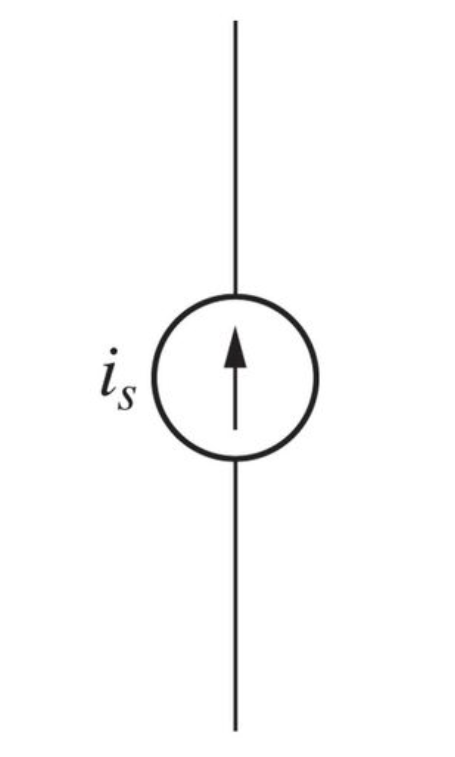
\includegraphics[width=\textwidth/2]{images/independentcurrentsource.png}
        \caption{Independent current source}
        \label{fig:independentcurrentsource}
    \end{marginfigure} 
    
\end{itemize}
Contrasted with independent sources are 
dependent sources. Dependent sources are sources 
whose values are 
dependent on other variables within the circuit. 
These sources are used to model components whose 
behavior changes according to the conditions in 
the circuit. There are four types of dependent sources:
\begin{itemize}
    \item \defn{Voltage-Controlled Voltage Source (VCVS)}{
    This type of dependent source generates a voltage 
    that is proportional to the voltage across a 
    separate part of the circuit.}
    \begin{marginfigure}
        \centering
        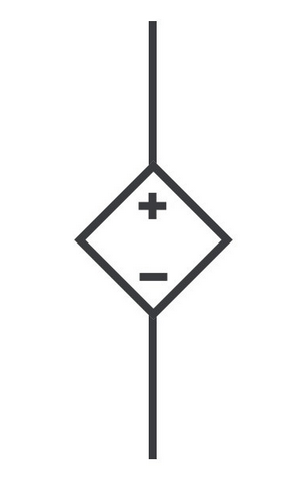
\includegraphics[width=\textwidth/2]{images/dependentvoltagesource.png}
        \caption{Dependent voltage source}
        \label{fig:dependentvoltagesource}
    \end{marginfigure} 

    \item \defn{Current-Controlled Current Source (CCCS)}{
    This type of dependent source generates a current 
    that is proportional to the current flowing 
    through a different part of the circuit.}
    \begin{marginfigure}
        \centering
        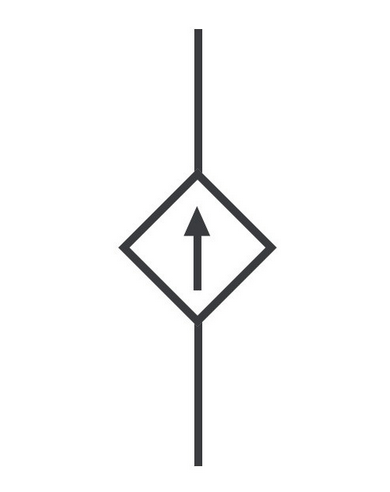
\includegraphics[width=\textwidth/2]{images/dependentcurrentsource.png}
        \caption{Dependent current source}
        \label{fig:dependentcurrentsource}
    \end{marginfigure} 


    \item \defn{Voltage-Controlled Current Source (VCCS)}{
    This type of dependent source generates a 
    current that is proportional to the 
    voltage across a different part of the 
    circuit.}
    \item \defn{Current-Controlled Voltage Source (CCVS)}{
    This type of dependent source generates a 
    voltage that is proportional to the 
    current flowing through a separate part 
    of the circuit.}
\end{itemize}
In both the independent and dependent case, we assume
the sources are ideal. There are two
critical attributes of ideal sources. First, their value remains unchanged indefi-
nitely. Second, they can deliver any amount of power needed by their loads.
Turning off a voltage source is equivalent to replacing it with a 
short circuit (line). Turning off a current source is equivalent to replacing it with an
open circuit (broken line). Also equivalent to an open
circuit is a resistor with infinite resistance. 
Resistance is a measure of how hard it is to shove current
through a resistor. The harder it is, the higher the
resistance. It's given by $R = \frac{\rho L}{A} = \frac{V}{I}$, where $\rho$ 
is the resistivity, $L$ is the length of the resistor, and $A$ is the 
cross-sectional area of the resistor. The reciprocal of
resistance is conductance ($G = \frac{1}{R}$). We can relate 
voltage, current and resistance with \emph{Ohm's Law}.

\defn{Ohm's Law}{$V = IR$.} This law is fundemental to EE and will
occur repeatedly throughout the course. 

\section{Kirchhoff's Laws, resistor combinations, and voltage/current division}
\defn{Kirchhoff's Current Law}{The sum of all currents going into
a node is 0. Mathematically, $\sum_k i_k = 0$}. We may intuit 
this by imagining electricity as water flowing into a pipe. Anything that flows 
in must flow out.
Say you have a circuit such as fig. \ref{fig:kcl}. 
\begin{figure}
    \center
    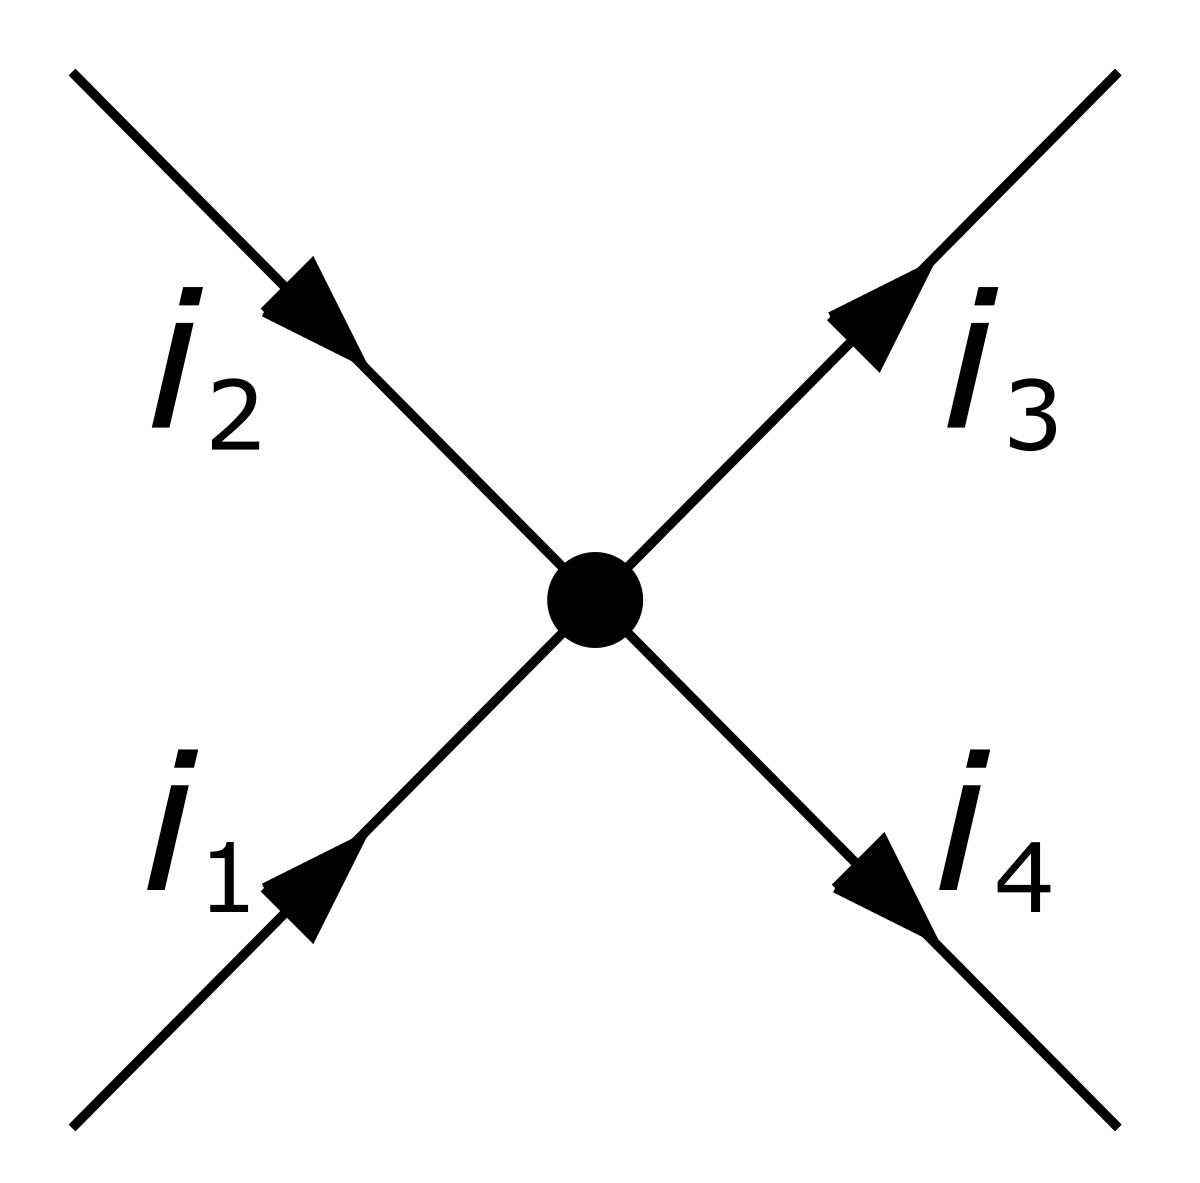
\includegraphics[width=\textwidth/2]{images/1200px-Kirchhoff's_Current_Law.svg.png}
    \caption{Kirchhoff's Current Law}
    \label{fig:kcl}
\end{figure}
By Kirchhoff's
current law, we see that $i_1+i_2-i_3-i_4 = 0 \rightarrow i_1 + i_2 = i_3 +i_4$.
The neat thing is that this must be true for any node in a circuit. 
If you have a node with two known currents going in and one unkown comming out,
Kirchhoff's current law tells us the unknown current is simply the sum
of the known currents. 

Contrasted with Kirchhoff's current law, we have Kirchhoff's voltage
law. 

\defn{Kirchhoff's Voltage Law}{In a closed loop, the sum
of all voltage drops is zero. Mathematically, $\sum_k v_k = 0$}.
A useful way to visualize this is to think of voltage as potential energy.
No matter where you go and how the voltage drops and rises, 
when you get back to where you began, the voltage must be the same
there. You end up with the same gravitational potential if
you return to the same spot, even if you run up and down a mountain.
Imagine a closed loop such as fig. \ref{fig:series}.
Say the voltage across the battery is $15V$ and each resistor
is identical. Although we don't know for sure yet, we can guess
that the current will be the same through each, and ergo
by Ohm's Law ($V=IR$) so will each voltage. Therefore,
\[15 + 3V = 0 \rightarrow V = -5\]

Now that we have a good idea of circuit components and how voltage/current behave, we can look 
at important configurations. These are the most useful:

\defn{Series Combination}{In a series combination, the elements 
are connected with end to end in contact}. We can use Kirchhoff's current
law to show that the current at each point in the circuit is the same. Since current 
flows into a resistor it has no option but to flow out the same resistor.
\begin{figure}
    \center
    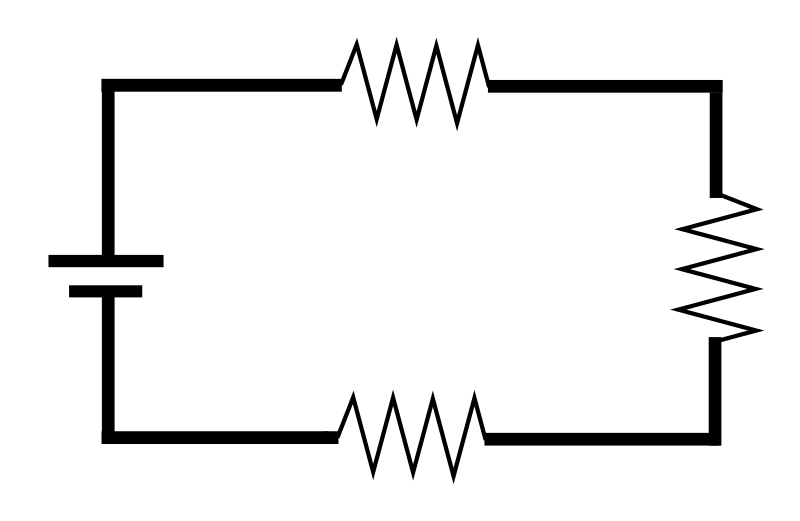
\includegraphics[width=\textwidth/2]{images/Series_circuit.svg.png}
    \caption{Series Combination}
    \label{fig:series}
\end{figure}
Say the resistances are $R_1, R_2$, and $R_3$. By Kirchhoff's voltage law, we have
\begin{align*}
    V &= IR_1 + IR_2 + IR_3\\
    &= I(R_1 + R_2 + R_3) \\
    &= IR_{total} \\
    &\rightarrow R_{total} = R_1 + R_2 + R_3\\
\end{align*}
Therefore for resistors in series, the total resistance is 
equal to the sum of each individual resistance. 

\defn{Parallel Combination}{When two or more resistances are 
connected between the same two points, they are said to be 
connected in parallel. Here, voltage is equal
across all elements}. 
\begin{figure}
    \center
    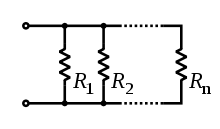
\includegraphics[width=\textwidth/2]{images/220px-Resistors_in_parallel.svg.png}
    \caption{Parallel Combination}
    \label{fig:parallel}
\end{figure}
In fig. \ref{fig:parallel}, the total current is split among
$n$ different resistors. That is, $I = \sum_k^n i_k$. With a bit of
manipulation and Ohm's Law, we have that
\begin{align*}
    I &= \frac{V}{R_{total}}\\
    &= \sum_k^n i_k \\
    &= \sum_k^n V/R_k \\
    &\rightarrow \frac{1}{R_{total}} \\
    &= \sum_k^n \frac{1}{R_k} \\
\end{align*}

So for resistors in parallel, the reciprocal of the total resistance is 
the sum of the reciprocals of the individual resistances. 

Now would
be an excellent point to introduce the idea of 

\section{Equivalent resistance}

\defn{Equivalent resistance}{a simplification
of a circuit with multiple resistors, where the resistance
of the equivalent resistor maintains the same voltage 
and current relationship.} We have already seen formulas
for when the resistors are in parallel or series, and can
use them to determine the equivalent resistance across two nodes.
For instance, consider fig. \ref{fig:seriesandparallelequi}.
\begin{figure}

    \caption{Finding equivalent resistance in circuit with 
    resistors in series and parallel, step 1}
    \center
    \label{fig:seriesandparallelequi}
    \begin{circuitikz}
        % Circuit code
        \draw (0,0)node[left=0.2cm]{B} 
            to[short,o-] ++(1,0) coordinate(b1) 
            to[short] ++(3,0) coordinate (b2) 
            to[short] ++ (2.5,0) 
            to[R,l_=$\SI{1.5}{\kilo\ohm}$] ++(0,2.5)  coordinate (c1) 
            to[R,l_=$\SI{3}{\kilo\ohm}$] ++(0,2.5) 
            to[short] ++(-2.5,0) coordinate (a2) 
            to[R,l_=$\SI{1}{\kilo\ohm}$]++(-3,0) coordinate (a1) 
            to[short,-o] ++(-1,0) node[left=0.2cm]{A} ;
         
        \draw (a1) to[R,l_=$\SI{10}{\kilo\ohm}$,*-*] (b1);
         
        %\draw (c1) to[R,l_=$\SI{5}{\kilo\ohm}$,*-] ++ (-2.5,0)coordinate (c2);
         
        \draw (c1) ++ (-2.5,0) to[R,l=$\SI{2}{\kilo\ohm}$,-*] (a2);
        \draw (c1) ++ (-2.5,0) to[R,l_=$\SI{5}{\kilo\ohm}$,*-*] (b2);
         
    \end{circuitikz}
\end{figure}
We can see that the $1 \Omega$ and the $10 \Omega$ resistor are in series, 
so their equivalent resistance is simply $1 + 10 \Omega = 11 \Omega$. We can condense the
circuit to fig \ref{fig:seriesandparallelequi2}. 
\begin{figure}

    \caption{Finding equivalent resistance in circuit with 
    resistors in series and parallel, step 2}
    \center
    \label{fig:seriesandparallelequi2}
    \begin{circuitikz}
        % Circuit code
        \draw (0,0)node[left=0.2cm]{B} 
            to[short,o-] ++(1,0) coordinate(b1) 
            to[short] ++(3,0) coordinate (b2) 
            to[short] ++ (2.5,0) 
            to[R,l_=$\SI{1.5}{\kilo\ohm}$] ++(0,2.5)  coordinate (c1) 
            to[R,l_=$\SI{3}{\kilo\ohm}$] ++(0,2.5) 
            to[short] ++(-2.5,0) coordinate (a2) 
            to[short] ++(-3,0) coordinate (a1)
            to[short,-o] ++(-1,0) node[left=0.2cm]{A} ;
         
        \draw (a1) to[R,l_=$\SI{11}{\kilo\ohm}$,*-*] (b1);
         
        \draw (c1) ++ (-2.5,0) to[R,l=$\SI{2}{\kilo\ohm}$,-*] (a2);
        \draw (c1) ++ (-2.5,0) to[R,l_=$\SI{5}{\kilo\ohm}$,*-*] (b2);
    \end{circuitikz}
\end{figure}
We next combine the $2 \Omega$ and the $5 \Omega$ resistor to obtain an
equivalent resistance of $7 \Omega$, and the $3 \Omega$ and the $1.5 \Omega$
to obtain $4.5 \Omega$ (fig. \ref{fig:seriesandparallelequi3})
\begin{figure}

    \caption{Finding equivalent resistance in circuit with 
    resistors in series and parallel, step 3}
    \center
    \label{fig:seriesandparallelequi3}
    \begin{circuitikz}
        % Circuit code
        \draw (0,0)node[left=0.2cm]{B} 
            to[short,o-] ++(1,0) coordinate(b1) 
            to[short] ++(3,0) coordinate (b2) 
            to[short] ++ (2.5,0) 
            to[R,l_=$\SI{1.5}{\kilo\ohm}$] ++(0,5)  coordinate (c1) 
            to[short] ++(-2.5,0) coordinate (a2) 
            to[short] ++(-3,0) coordinate (a1)
            to[short,-o] ++(-1,0) node[left=0.2cm]{A} ;
         
        \draw (a1) to[R,l_=$\SI{11}{\kilo\ohm}$,*-*] (b1);
         
        \draw (c1) ++ (-2.5,0) to[R,l=$\SI{2}{\kilo\ohm}$,-*] (b2);
    \end{circuitikz}
\end{figure}
Now that we are left with only resistors in parallel, we may use the formula
$\frac{1}{R_{eq}} = \sum_k \frac{1}{R_k}$ to obtain 
$\frac{1}{R_eq} = \frac{1}{11} + \frac{1}{2} + \frac{1}{1.5} = \frac{83}{66}$,
yielding $R_{eq} = \frac{66}{83} \Omega$. 
Note that this method is only possible when the circuit has 
resistors in series or parallel. For more complex situations, such as
when souces are present or resistors are combined in neither
series nor parallel, we must use Kirchhoff's laws and good judgement 
to find the equivalent resistance. Consider fig. \ref{fig:eqresources}, where 
we have a circuit with both dependent and independent sources. 
\begin{figure}
    \caption{Finding equivalent resistance in cirucit with sources}
    \label{fig:eqresources}
    \begin{circuitikz}[american currents, american voltages]
        % Circuit code
        \draw (0,0)node[left=0.2cm]{B}
            to[short,o-] ++(0.5,0) coordinate (b1)
            to[short,] ++(2,0) coordinate (b2)
            ;
        \draw (0,2)node[left=0.2cm]{A}
            to[short,o-] ++(0.5,0) coordinate (a1)
            ;
        \draw to[short] (b1) (a1)
            (b1) to[I, l_=$3A$] (a1)
            ;
        \draw (a1) to[short] ++ (0.5,0) 
            to[R,l^=$\SI{4}{\ohm}$, v_>=$V_1$] ++(1,0)   
            to[short] ++ (0.5,0) coordinate (a2)
            ;
        \draw (b2) to [cI, l_=$(0.25 S) V_1$] (a2);
        \draw (a2) to[short] ++(3,0) coordinate (a3)
            (a3) to[R,l^=$\SI{8}{\ohm}$] ++(0,-2) coordinate (b3)
            (b3) to[short] (b2)
            ;
    \end{circuitikz}
\end{figure}
The process for finding the equivalent resistance of a circuit 
with sources is as follows:
\begin{enumerate}
    \item "Turn off" all independent sources. That is, replace independent current sources with
    opens and independent voltage sources with shorts. 
    \item Apply a test current or voltage across $a$ and $b$.
    \item Use $R_{eq} = \frac{V_test}{I_test}$, circuit laws, and algebra to solve. 
\end{enumerate}
Let's apply a test current of $1 A$ across $a,b$, as shown in fig. \ref{fig:eqresources2}
\begin{figure}
    \caption{Finding equivalent resistance in cirucit with sources}
    \label{fig:eqresources2}
    \begin{circuitikz}[american currents, american voltages]
        % Circuit code
        \draw (0,0)node[left=0.2cm]{B}
            to[short,o-] ++(0.5,0) coordinate (b1)
            to[short,] ++(2,0) coordinate (b2)
            ;
        \draw (0,2)node[left=0.2cm]{A}
            to[short,o-] ++(0.5,0) coordinate (a1)
            ;
        \draw (0,0) to[I, l_=$3A$] (0,2);
        \draw (a1) to[short] ++ (0.5,0) 
            to[R,l^=$\SI{4}{\ohm}$, v_>=$V_1$] ++(1,0)   
            to[short] ++ (0.5,0) coordinate (a2)
            ;
        \draw (b2) to [cI, l_=$(0.25 S) V_1$] (a2);
        \draw (a2) to[short] ++(3,0) coordinate (a3)
            (a3) to[R,l^=$\SI{8}{\ohm}$] ++(0,-2) coordinate (b3)
            (b3) to[short] (b2)
            ;
        \draw (a2) node[above]{x};
        \draw (a3) to [short,i>=$I_y$] ++(0,-0.25);
    \end{circuitikz}
\end{figure}
By using Kirchhoff's voltage law
on the outermost loop, we have 
\[V_{test} = V_1 + 8 I_y\]
We also know that the current flowing into node $x$ must be 
equal to the current flowing out. That is, 
\[1 + (0.25 S)V_1 =I_y\]
But since we know $R_1$ and $I_1$, we can find $V_i$. We simply have 
\[V_1 = 1 A \times 4 \Omega = 4 V\]
Meaning 
\[I_y = 4 * 0.25 + 1 = 2\]
We can plug $V_1$ and $I_y$ into $V_{test} = V_1 + 8 I_y$ to get $V_{test} = 4 + 16 = 20$,
and via $R_{eq} = \frac{V_{test}}{I_{test}}$ we have $R_{eq} = \frac{20 V}{1 A} = 20 \Omega$.

\section{Analysis}
Let's now examine a couple of extremely powerful techniques we can use 
to analyze circuits, \emph{nodal analysis} and \emph{mesh analysis}.  

\defn{Nodal analysis}{a systematic method used to determine the voltage at every 
(essential) node in a circuit. After picking our reference (ground) node, we
systematically apply KCL at every (essential) node in the circuit except,
of course, for the ground node. By finding every nodal voltage in the circuit, 
we can find every branch current, which enables us to determine the
power absorbed or delivered by every element. Because of its ability to
be applied to any circuit, nodal analysis is the method most often used
in circuit analysis computer programs}. Here are the steps to perform nodal 
analysis: 
\begin{enumerate}
    \item Number all (essential) nodes of the given circuit.
    \item Write KCL for every (essential) node by keeping in mind that only nodal
    voltages should be used (no currents). If other unknowns are involved (e.g.
    dependent source equations) express them as a function of the unknown
    nodal voltages (e.g. by using Ohm's law).
    \item Group the resulting equations together in a matrix form.
    \item Solve for the unknown nodal voltages by inverting the resulting linear
    equation.
    \item Calculate any quantity of interest (e.g power consumption) from the
    known nodal voltages.
\end{enumerate}
Consider an example cirucit, fig. \ref{fig:nodalanal}.
\begin{figure}
    \caption{Using nodal analysis}
    \label{fig:nodalanal}
    \begin{circuitikz}[american currents, american voltages]
        \draw (0,0) to[I, l_=$I_{s_1}$] (0,3) coordinate (a1)
            to[short,-o] ++(2,0) coordinate (a2)
            to[R, l=$R_2$] ++(2,0) coordinate (a3)
            to[short] ++(2,0) coordinate (a4)
            to[V, l=$V_{s_3}$] ++(0,-3) coordinate (b4)
            (b4) to (3,0) node[ground]{}
            (3,0) to[short] (0,0)
            (a2) to[R, l=$R_1$] (2,0)
            (a3) to[I, l=$I_{s_2}$] (4,0)
            ;
        \draw (a2) node[above]{$V_1$};
        \draw (a3) node[above]{$V_2$};
    \end{circuitikz}
\end{figure}
Let's apply our steps to find the nodal voltages $V_1$ and $V_2$.
\begin{enumerate}
    \item Number the essential nodes (fig. \ref{fig:nodalanal2}).
    \begin{figure}
        \caption{Numbering nodes}
        \label{fig:nodalanal2}
        \begin{circuitikz}[american currents, american voltages]
            \draw (0,0) to[I, l_=$I_{s_1}$] (0,3) coordinate (a1)
                to[short,-o] ++(2,0) coordinate (a2)
                to[R, l=$R_2$] ++(2,0) coordinate (a3)
                to[short] ++(2,0) coordinate (a4)
                to[V, l=$V_{s_3}$] ++(0,-3) coordinate (b4)
                (b4) to (3,0) node[ground]{}
                (3,0) to[short] (0,0)
                (a2) to[R, l=$R_1$] (2,0)
                (a3) to[I, l=$I_{s_2}$] (4,0)
                ;
            \draw (a2) node[above]{1};
            \draw (a3) node[above]{2};
        \end{circuitikz}
    \end{figure}
    \item Apply Kirchhoff's current law to each node
    \begin{align*}
        -I_{s_1} - \frac{0-V_1}{R_1} - \frac{V_2-V_1}{R_2} &= 0\\
    \end{align*}
    Here we can actually take a shortcut. Since the negative terminal 
    of $V_{s_3}$ is grounded, then the voltage at the positive terminal 
    must be $V_{s_3}$. Since this terminal is connected directly to $V_2$, 
    we know that $V_2 = V_{s_3}$. That makes our equations
    \begin{align*}
        -I_{s_1} - \frac{0-V_1}{R_1} - \frac{V_2-V_1}{R_2} &= 0\\
        V_2 &= V_{s_3} \\
    \end{align*}
    \item Let's group these by the variables we wish to find now. 
    \begin{align*}
        V_1(\frac{1}{R_1} + \frac{1}{R_2}) - V_2\frac{1}{R_2} &= I_{s_1}\\
        0V_1 + V_2 &= V_{s_3} \\
    \end{align*}
    Which in matrix form becomes
    \[ \begin{bmatrix}
        \frac{1}{R_1} + \frac{1}{R_2} & -\frac{1}{R_2} \\
        0 & 1
    \end{bmatrix}
    \begin{bmatrix}
        V_1 \\
        V_2
    \end{bmatrix}
     =
    \begin{bmatrix}
        I_{s_1} \\
        V_{s_3}
    \end{bmatrix} \]
    \item From here, we could use a computer program to find the inverse matrix
    and multiply both sides by it to get the vector [$V_1$, $V_2$] by itself. 
    I'm not going to do this because I'm lazy, but if you're interested try 
    using Mathematica or MATLAB. 
\end{enumerate}

If our circuit lacks a ground, we may simply choose some node as ground, since
voltages are relative and having a grounded node makes analysis easier. 

%Super nodes?

%Modified nodal analysis

\defn{Mesh analysis}{This method is used to determine every loop current in a circuit. We
use KVL around meshes (loops) to find the mesh (loop) currents. We
can then calculate any voltage or any branch current from the resulting
mesh currents. (Basic) mesh analysis has a limitation in that it can only
be applied to planar circuits}.

Here are the steps to perform mesh analysis: 
\begin{enumerate}
    \item Choose your loops and draw mesh currents in them. 
    \item Use Kirchhoff's voltage law and the voltages you encounter 
    to create a system of equations. If two mesh currents 
    go against each other, the net current is their difference. 
    \item Group the resulting equations together in a matrix form.
    \item Solve for any quantity of interest. 
\end{enumerate}

Note that you don't want two mesh currents flowing through the same 
current source. If you find a circuit where this occurs, make a 
larger loop where no current sources are shared. 

\section{Source transformations}
\defn{Source transformation}{Source transformation is a 
wonderful tool that can be used to change the
originally given circuit to an equivalent and simpler circuit}.
Two important theorems are Thevenin's theorem and Norton's theorem.

\defn{Thevenin's theorem}{states that it 
is possible to simplify any linear circuit, irrespective of 
how complex it is, to an equivalent circuit with a single 
voltage source and a series resistance}. 

\begin{figure}
    \caption{Thevenin equivalent}
    \label{fig:thevenin}
    \begin{circuitikz}[american currents, american voltages]
        \draw (0,0) to[V, v=$V_{s}$, invert] (0,3) coordinate (a1)
            to[R, l=$R_s$, -o] ++(2,0) coordinate (a2);
        \draw (0,0) to[short, -o] (2,0);
    \end{circuitikz}
\end{figure}

\defn{Norton's theorem}{states that any 
linear circuit can be simplified to an equivalent circuit 
consisting of a single current source and parallel resistance 
that is connected to a load}.
\begin{figure}
    \caption{Norton equivalent}
    \label{fig:norton}
    \begin{circuitikz}[american currents, american voltages]
        \begin{circuitikz}[american currents, american voltages]
            \draw (0,0) to[I, l_=$I$] (0,3) coordinate (a1)
                to[short] ++(2,0) coordinate (a2);
            \draw (0,0) to[short] (2,0)
                to[R, l=$R_t$] ++(0,3);
            \draw (2,3) to[short, -o] (3,3);
            \draw (0,0) to[short, -o] (3,0);
        \end{circuitikz}
    \end{circuitikz}
\end{figure}
Let's see how to transform between these two. Fig. \ref{fig:tnsimp}
shows a circuit with one voltage source and a resistor in series. 
\begin{figure}
    \caption{Simple case of equivalency}
    \label{fig:tnsimp}
    \begin{circuitikz}[american currents, american voltages]
        \draw (0,0) to[V, v=$V_{s}$, invert] (0,3) coordinate (a1)
            to[R, l=$R_s$, -o] ++(2,0) coordinate (a2);
        \draw (0,0) to[short, -o] (2,0);
    \end{circuitikz}
\end{figure}
This series resistance normally represents the internal 
resistance of a practical voltage source.
Let us short circuit the output terminals of the 
voltage source circuit as shown in fig. \ref{fig:tnsimp2}
\begin{figure}
    \caption{Simple case of equivalency}
    \label{fig:tnsimp2}
    \begin{circuitikz}[american currents, american voltages]
        \begin{circuitikz}[american currents, american voltages]
            \draw (0,0) to[V, v=$V_{s}$, invert] (0,3) coordinate (a1)
                to[R, l=$R_s$, -o] ++(2,0) coordinate (a2);
            \draw (0,0) to[short, -o] (2,0)
                to[short] ++(0,3);
                ;
        \end{circuitikz}
    \end{circuitikz}
\end{figure}
We know that $V_s = I R_s$, where $I$ is the current delivered
by the voltage source when it is short circuited.
Now, let's take a current source of the same current $I$ 
which produces same open-circuit voltage at its open terminals 
as shown in fig. \ref{fig:tnsimp3}
\begin{figure}
    \caption{Simple case of equivalency}
    \label{fig:tnsimp3}
    \begin{circuitikz}[american currents, american voltages]
        \begin{circuitikz}[american currents, american voltages]
            \draw (0,0) to[I, l_=$I$] (0,3) coordinate (a1)
                to[short] ++(2,0) coordinate (a2);
            \draw (0,0) to[short] (2,0)
                to[R, l=$R_t$] ++(0,3);
            \draw (2,3) to[short, -o] (3,3);
            \draw (0,0) to[short, -o] (3,0);
        \end{circuitikz}
    \end{circuitikz}
\end{figure}
Now we have $I = \frac{V_s}{R_t}$, meaning $R_s = R_t$. The open circuit 
voltage of both the sources is $V_s$ and short 
circuit current of both sources is $I$. The 
same resistance connected in series in voltage 
source is connected in parallel in its equivalent current source.
So, the voltage source and current source are equivalent to each other.
Changing between forms is called a source transformation and can be used 
to simplify an electric circuit. 
\end{document}
